\chapter{Background} \label{Chapter:Background}

\section{Game Theory}

\subsection{Nash Equilibrium}
The concept of a Nash Equilibrium plays a central role in game theory. The definition in simple setting of a finite player is described as follow with mathematical form. Form indexes $K$ agents as $k=i, \dots, K$. There are total $N_k$ pure strategies. From $N_k$ agent k choose a strategy called $s_k$. $S_k$ denotes the set of strategies, and $s_k$ as the member of the set. A strategy profile, named $s = (s_1, ..., s_K)$, is a vector of strategies for the individual players. Hence, all strategy profiles can be written as $S$ for $\Pi_{k=1}^{K} S_{k}$. $s \mid s_{k}^{\prime}$ for the strategy $\left(s_{1}, \ldots, s_{k-1}, s_{k+1}^{\prime}, \ldots, s_{K}\right)$ means a strategy of agent $k$ changed from $s_k$ to $s_{k}^{\prime}$, in which a strategy profile $s$ is $s = (s_1, ..., s_K)$ and a strategy of agent $k$ is $s_{k}^{\prime} \in S_{k}$. The excepted utility or payoff of each agent $k$ is formed as $u_k(s)$, when agents select strategy profile $s$.

I players indexed by i=1,...,I. The strategy of agent i is si choosed from Ni pure strategies. A strategy profile of all agents written as s = (s1, s2, sI), si|si' for the strategy profile (s1, ... si-1, si+1, sI), or the s with the part of i changed from si to si'. For each player i and strategy s, ui(s) denotes i's expected utility[]. 

\begin{proposition}[Nash Equilibrium]
For a strategy profile $s$, Nash Equilibrium can be described for each agent $k$ and $s_{k}^{\prime} \in S_{k}$, $u_{k}(s) \geqslant u_{k}\left(s \mid s_{k}^{\prime}\right)$
\end{proposition}

In terms of words description, the definition of Nash equilibrium is that if other agents do not change its strategy, then no single agent can obtain higher utility. 

The learning process of RL-Agent in this paper can be considered as an incomplete information static non-cooperative game.
 
\subsection{Pareto Efficient}

\begin{proposition}[Pareto Efficient]
no other feasible allocation $\{x_{1}',...,x_{n}'\}$ where, for 
utility function $u_i$ for each agent $i$, $u_{i}(x_{i})$ for all $i\in \{1,...,n\}$ with $u_{i}(x_{i}')>u_{i}(x_{i})$ for some $i$[].
\end{proposition}

Pareto Efficient is a state at which resources in a system are optimized in a way that one dimension cannot improve without a second worsening. 

\subsection{Markov Games}
\paragraph{Finite Markov Decision Processes}

\paragraph{Multi-Agent Markov Decision Processes} Methods mentioned in the paper are based on a multi-agent extension of Markov decision processes(\gls{mdps}) called partially observable Markov games. There are N players indexed by $n=1,2,...,N$.

\section{Autonomous Negotiaion} \label{autonomous-negotiation}
Negotiation is an important process in coordinating behavior and represents a principal topic in the field of multi-agent system research. There has been extensive research in the area of automated negotiating agents. 

Automated agents can be used side-by-side with a human negotiator embarking on an important negotiation task. They can alleviate some of the effort required of people during negotiations and also assist people who are less qualified in the negotiation process. There may even be situations in which automated negotiators can replace the human negotiators. Thus, success in developing an automated agent with negotiation capabilities
has great advantages and implications[].

Through the negotiation agents, many problems that arise in real or simulated domain can be solved. 
In industrial domains, 
In commerical  domains, the Supply Chain Management System (SCMS)
functionality is implemented through agent-based negotiation environment, in which contracts can be singed through negotiation between agents. Many papers describe ongoing effort in developing a Multi-agent System (MAS) for supply chain management[\gls{scml}].

In game domains, bilateral negotiation in [GENIUS]

\subsection{Utility Function}
Utility function is an important concept in economics. It measures preferences over a set of goods and services. Utility represents the satisfaction that consumers receive for choosing and consuming a product or service[]. In NegMAS and SCML, utility function could measure either single offer or set of offers.

Utility is measured in units called utils, but calculating the benefit or satisfaction that consumers receive from is abstract and difficult to pinpoint[]. In the package NegMAS, SCML are built-in some utility functions, through inheritance of these it is easy to design new Utility function by developer. Such as linear utiliy function and real utility function OneShotUfun designed in SCMLOneShotWorld.

[1] linear utility function
[2] real utility function OneShotUfun

It is a important point for designing a new Agent in autonomous negotiation environments. For heuristic agents utility function is a keypoint to measure preferences. For reinforment learning agents utiliy function conducts the behavior of learnable agents, used as a part of reward function, significantly affect the design and evaluation of RL-Agent.

\subsection{Rubinstein bargaining mechanism}
Rubinstein bargaining mechanism is widely cited for multi-round bilateral negotiation \parencite{Rubinstein1982}.
Two agents in the mechanism which has an infinite time horizon have to reach an agreement. 

To the state of nash equilibrium.

\subsection{Stacked alternating offers mechanism(SAOM)} \label{background:saom}
\gls{saom} is also named as stacked alternating offers protocol. Agents can only take their action when it is their turn. SAOM allows negotiating agents to evaluate only the most recent offer in their turn and accordingly they can either accept offer, make a count offer or walk away.

In the SCML OneShotWord, at the first step all of the agents will propose a first offer.

\section{Artificial Intelligence}
Artificial Intelligence is a broad branch of computer science that is focused on a machine’s capability to produce rational behavior from external inputs. The goal of AI is to create systems that can perform tasks that would otherwise require human intelligence[].

There is a set of three related items that sometimes are erroneously used interchangeably, namely artificial intelligence, machine learning, and neural networks. According to Encyclopaedia Britannica, AI defines the ability of a digital computer or computer-controlled robot to perform tasks commonly associated with intelligent beings. On the other hand, according to H.A. Simon, one of the pioneers of the field, machine learning is a “field of study that gives computers the ability to learn without being explicitly programmed”

\subsection{Sub-areas}
Fig. \ref{fig:ai_taxonomy} shows the relationship of artificial intelligence, machine learning and deep learning.
\begin{figure}[htbp]
\centering
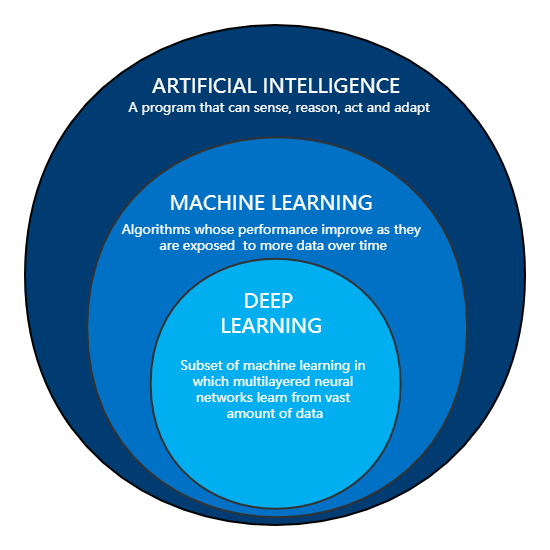
\includegraphics[width=0.4\textwidth]{./images/ai_taxonomy.png}
\caption{Sub-areas of artificial intelligence Source: Own illustration based
on\parencite{Suman2020}}
\label{fig:ai_taxonomy}
\end{figure}

\subsubsection{Artificial Intelligence}
Artificial intelligence, also called machine intelligence, can be understood by an intelligence, unlike the natural intelligence shown by humans and animals, which is demonstrated by machines. It looks at ways of designing intelligent devices and systems that can address problems creatively that are often treated as a human prerogative. Thus, AI means that a machine somehow imitates human behavior.
\subsubsection{Machine Learning} 
Machine learning is an AI subset and consists of techniques that enable computers to recognize data and supply AI applications. Different algorithms (e.g., neural networks) contribute to problem resolution in ML.
\subsubsection{Deep Learning}
Deep learning, often called deep neural learning or deep neural network, is a subset of machine learning that uses neural networks to evaluate various factors with a similar framework to a human neural system. It has networks that can learn from unstructured or unlabeled data without supervision.

\subsection{Methods}
\paragraph{Supervised Learning}
Training data contains optimal outcomes (also known as inductive learning). Learning is tracked in this method. Some famous examples of supervised machine learning algorithms are Linear regression for regression problems. 
\paragraph{Unsupervised Learning} 
There are not the desired outputs in the training results. Clustering is an example. It is impossible to know what is and what is not good learning.
\paragraph{Semi-supervised Learning}
A few desired outputs are included in the training data.
\paragraph{Reinforcement Learning}
Rewards are given after a sequence of actions. In a given case, it is a matter of taking appropriate steps to maximize compensation. It is the most ambitious method of learning in AI.

\subsection{Application Field}
Artificial intelligence (AI) researchers have paid a great deal of attention to automated negotiation over the past decade and a number of prominent models have been proposed in the literature. Autonomous Agent is an important concept of AI.
Artificial intelligence is a big concept with a wide range of applications. It provides support for many scenarios, such as eCommerce, Logistics and Supply Chain and as research tools for computer science.

\subsubsection{eCommerce}
\paragraph{Rank in E-Commerce Search Engine} In E-commerce platforms such as Amazon and TaoBao, ranking items in a search session is a typical multi-step decision-making problem. AI can learn the relation between different ranking steps, in the paper
\parencite{Hu2018} authors use reinforcement learning (RL) to learn an optimal ranking policy which maximizes the expected accumulative rewards in a search session. The more reasonable the ranking of commodities, the more frequent commodity transactions, and the greater the corresponding income.

\paragraph{Business-to-Business Negotiation} Negotiation is an important challenge for B2B e-commerce \parencite{Hans01}. For B2B e-commerce, artificial intelligence is making great strides and is being used in a variety of ways to improve and enhance business. AI-based algorithms and tools can help companies in a variety of ways, from personalizing the shopping experience to improving supply chain management.

\subsubsection{Logistics and Supply Chain}
\paragraph{Contextual Intelligence} Artificial intelligence provides contextual intelligence for the supply chain, they can use contextual intelligence to reduce operating costs and manage inventory. Contextual information helps them return to customers quickly.  
\paragraph{Enhancing Productivity and Profits} Artificial intelligence can analyze the performance of the supply chain and propose new factors that affect the same field. It can combine the capabilities of different technologies such as reinforcement learning, unsupervised learning and supervised learning to discover factors and problems that affect the performance of the supply chain and can make better contracts between different suppliers and consumers\parencite{Pndey2019}. It can analyze the data related to the supplier like audits, in-full delivery performance, credit scoring, evaluations and based on that deliver information which can be used to make future decisions. This kind of step helps the company make better decisions as a supplier and work towards improving customer service. Autonomous Negotiation by autonomous agent is an important concept that can be used in this field. 

\subsubsection{Tools for computer science}

\section{Artificial Neural Network}
Artificial neural network is a technology based on the study of the brain and nervous system\parencite{WALCZAK2003631}, as shown in Figure \ref{}. ANNs are efficient data-driven modelling tools widely used for nonlinear systems dynamic modelling and identification, due to their universal approximation capabilities and flexible structure that allow to capture complex nonlinear behaviors \parencite{SHOKRY2018265}. 



\subsection{Artificial Neuron}
Artifical neuron is shown in Figure \ref{fig:neuron}

\begin{figure}[htbp]
\centering
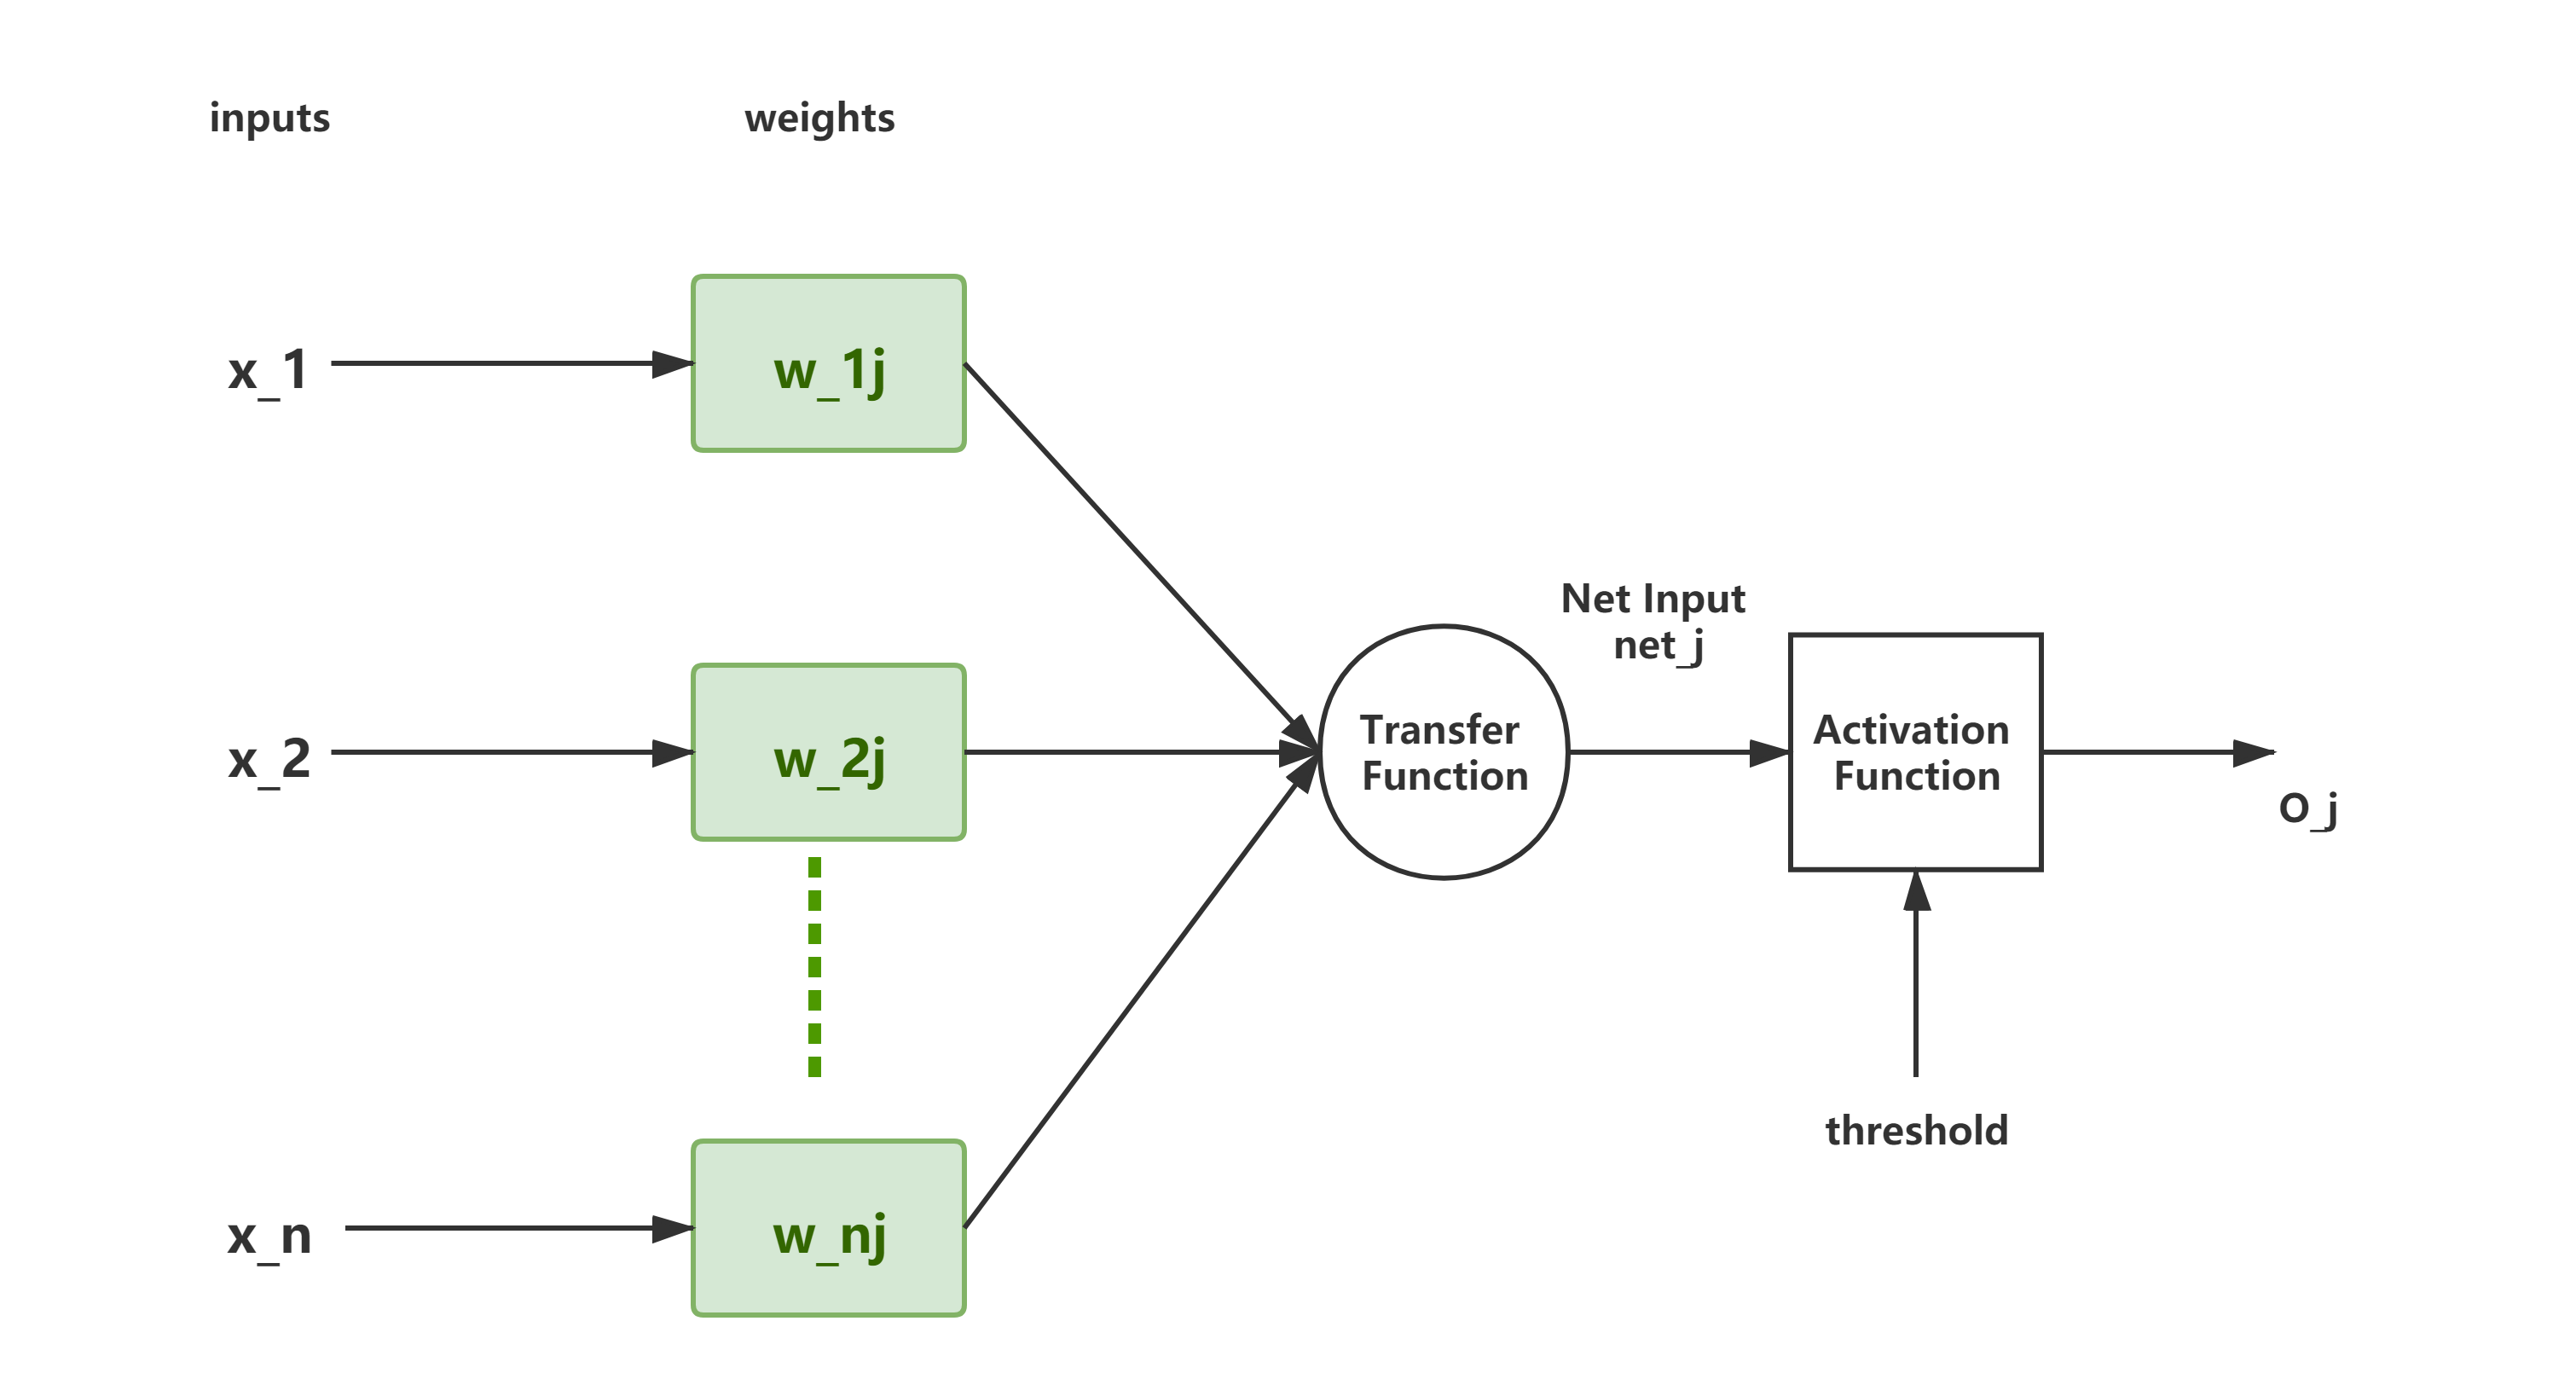
\includegraphics[width=0.9\textwidth]{./images/neuron.png}
\caption{Aritifical Neuron}
\label{fig:neuron}
\end{figure}

\subsection{Multi-Layers Neural Networks}
Figure \ref{fig:multi-layer-ann} diagrams the multi-layers neural networks.

\begin{figure}[htbp]
\centering
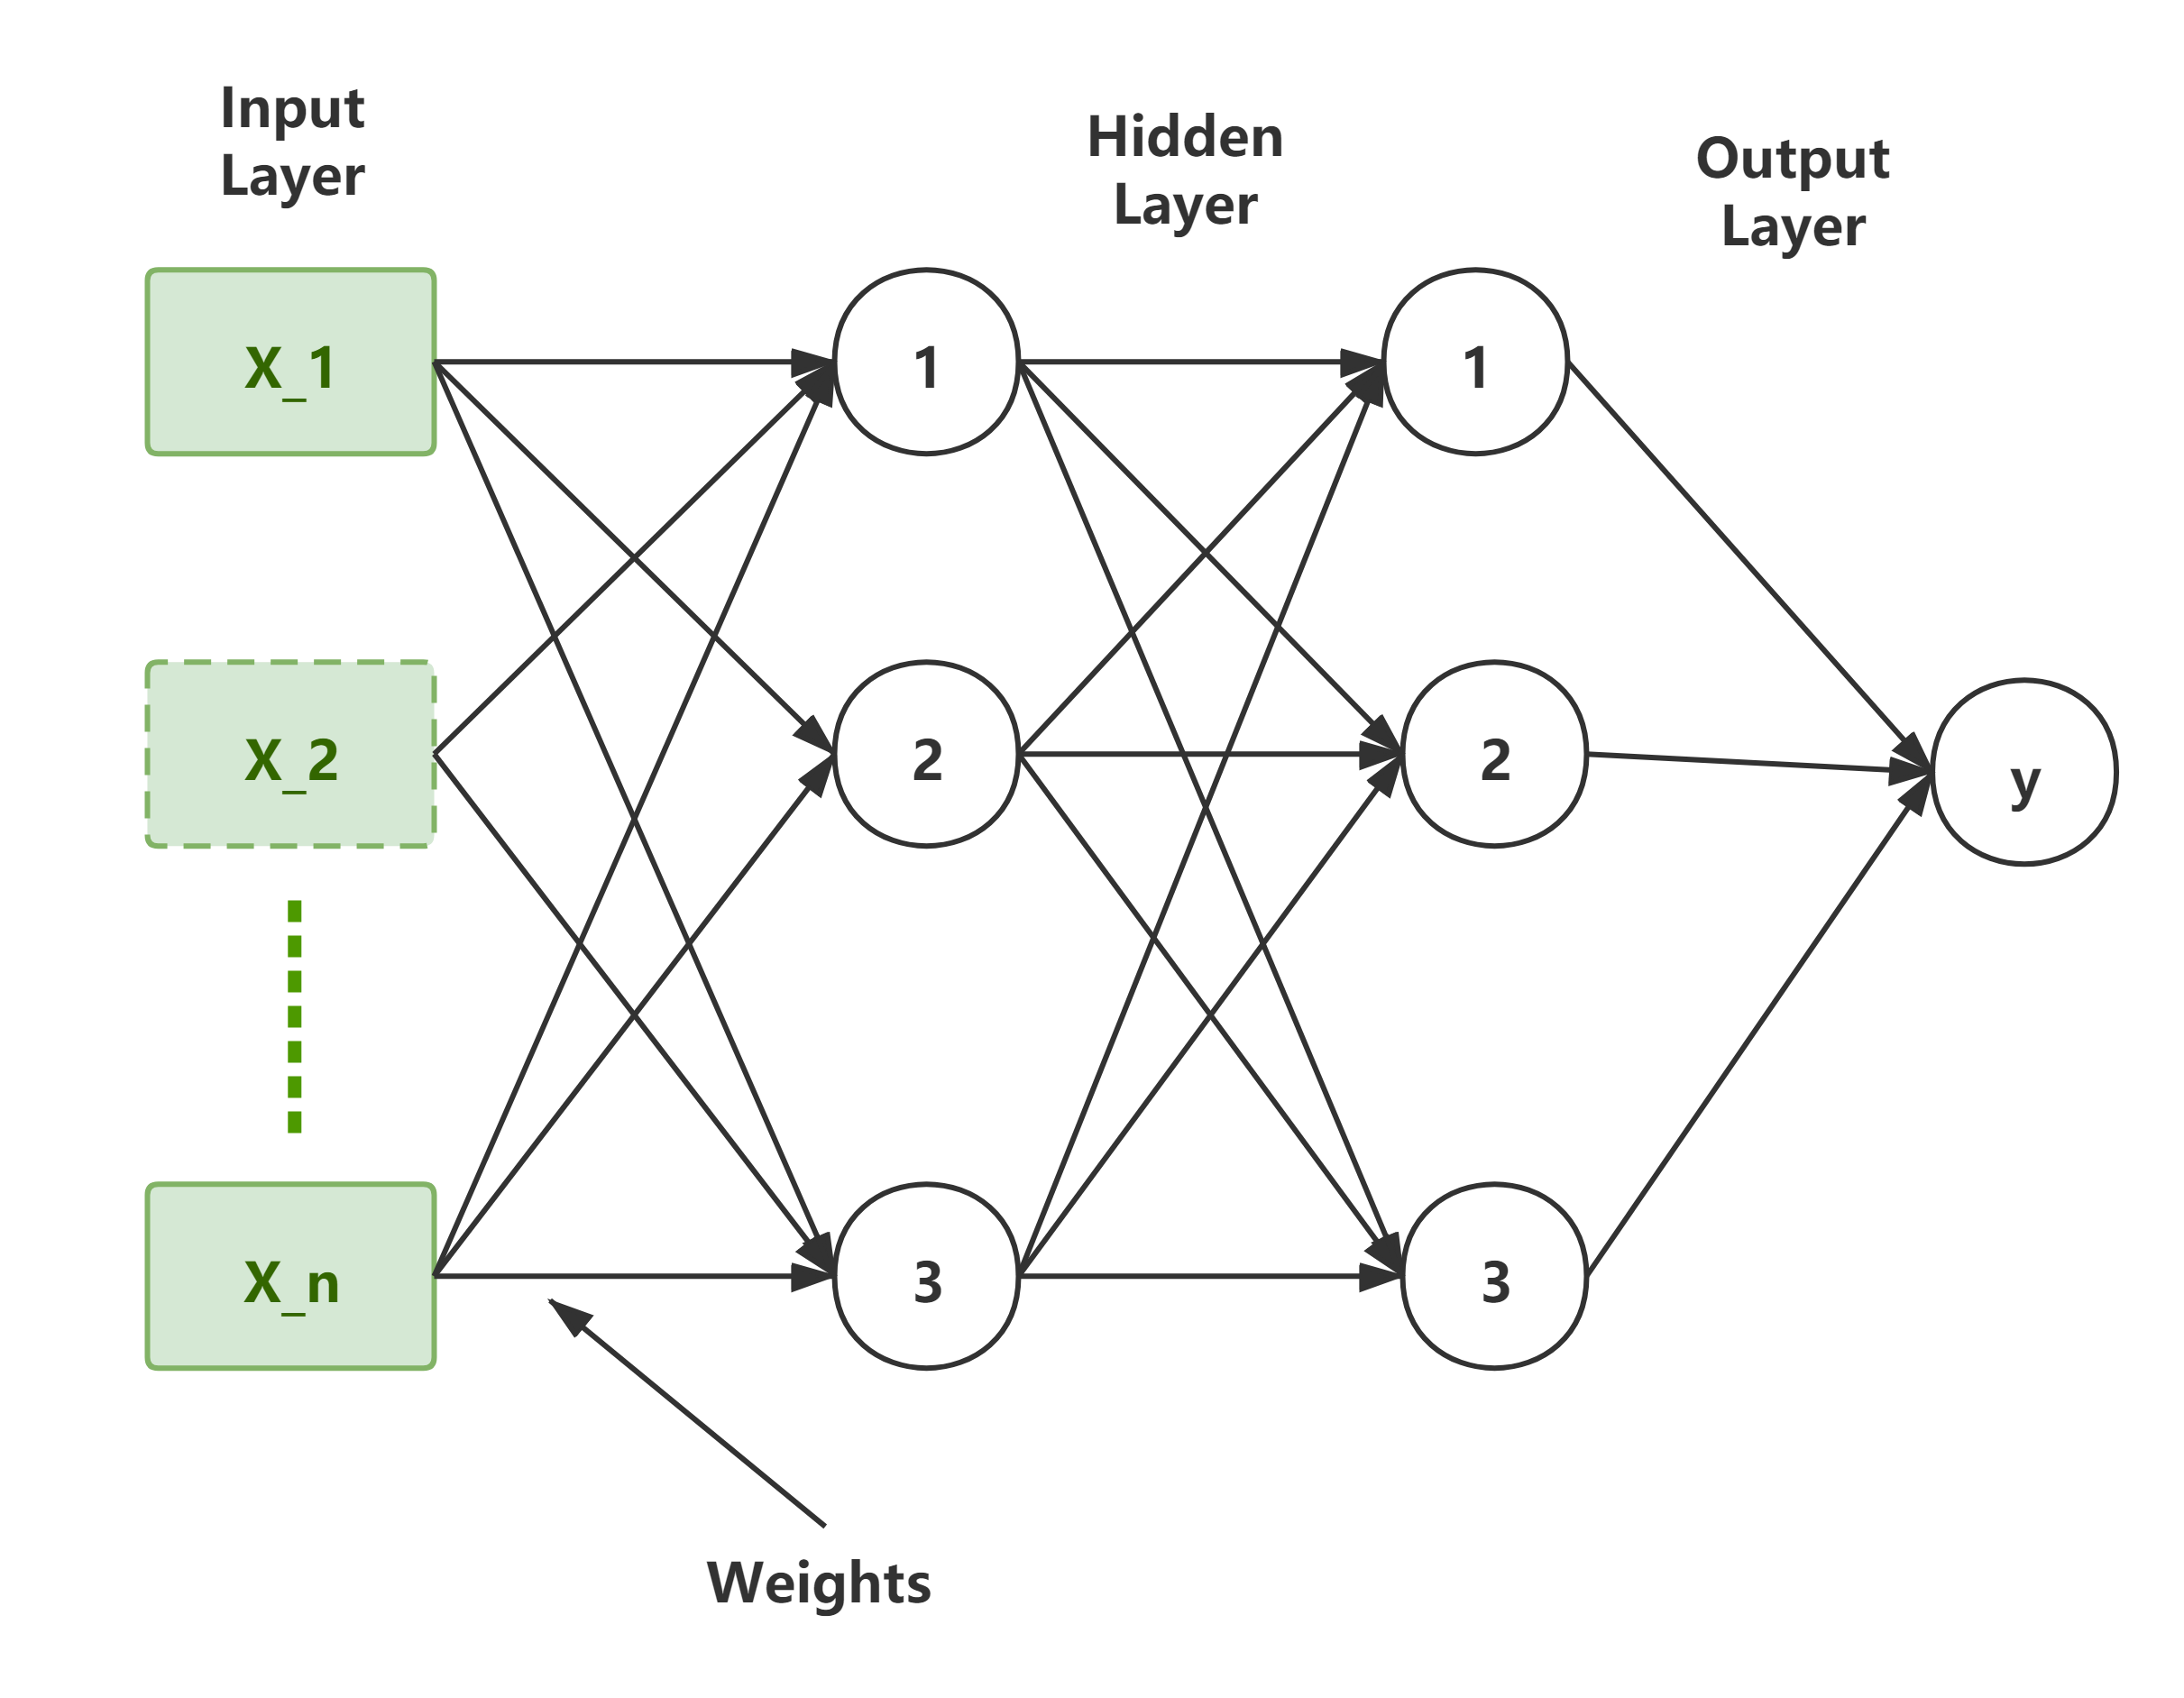
\includegraphics[width=0.9\textwidth]{./images/multi-layer-ann.png}
\caption{Aritifical Multi-Layers Neural Network, Source: Own illustration based
on\parencite{SAIRAMYA2019253}}
\label{fig:multi-layer-ann}
\end{figure}

\subsection{Recurrent Neural Networks (RNNS)}
Figure \ref{fig:recurrent-layer-ann} diagrams the recurrent neural networks.

\begin{figure}[htbp]
\centering
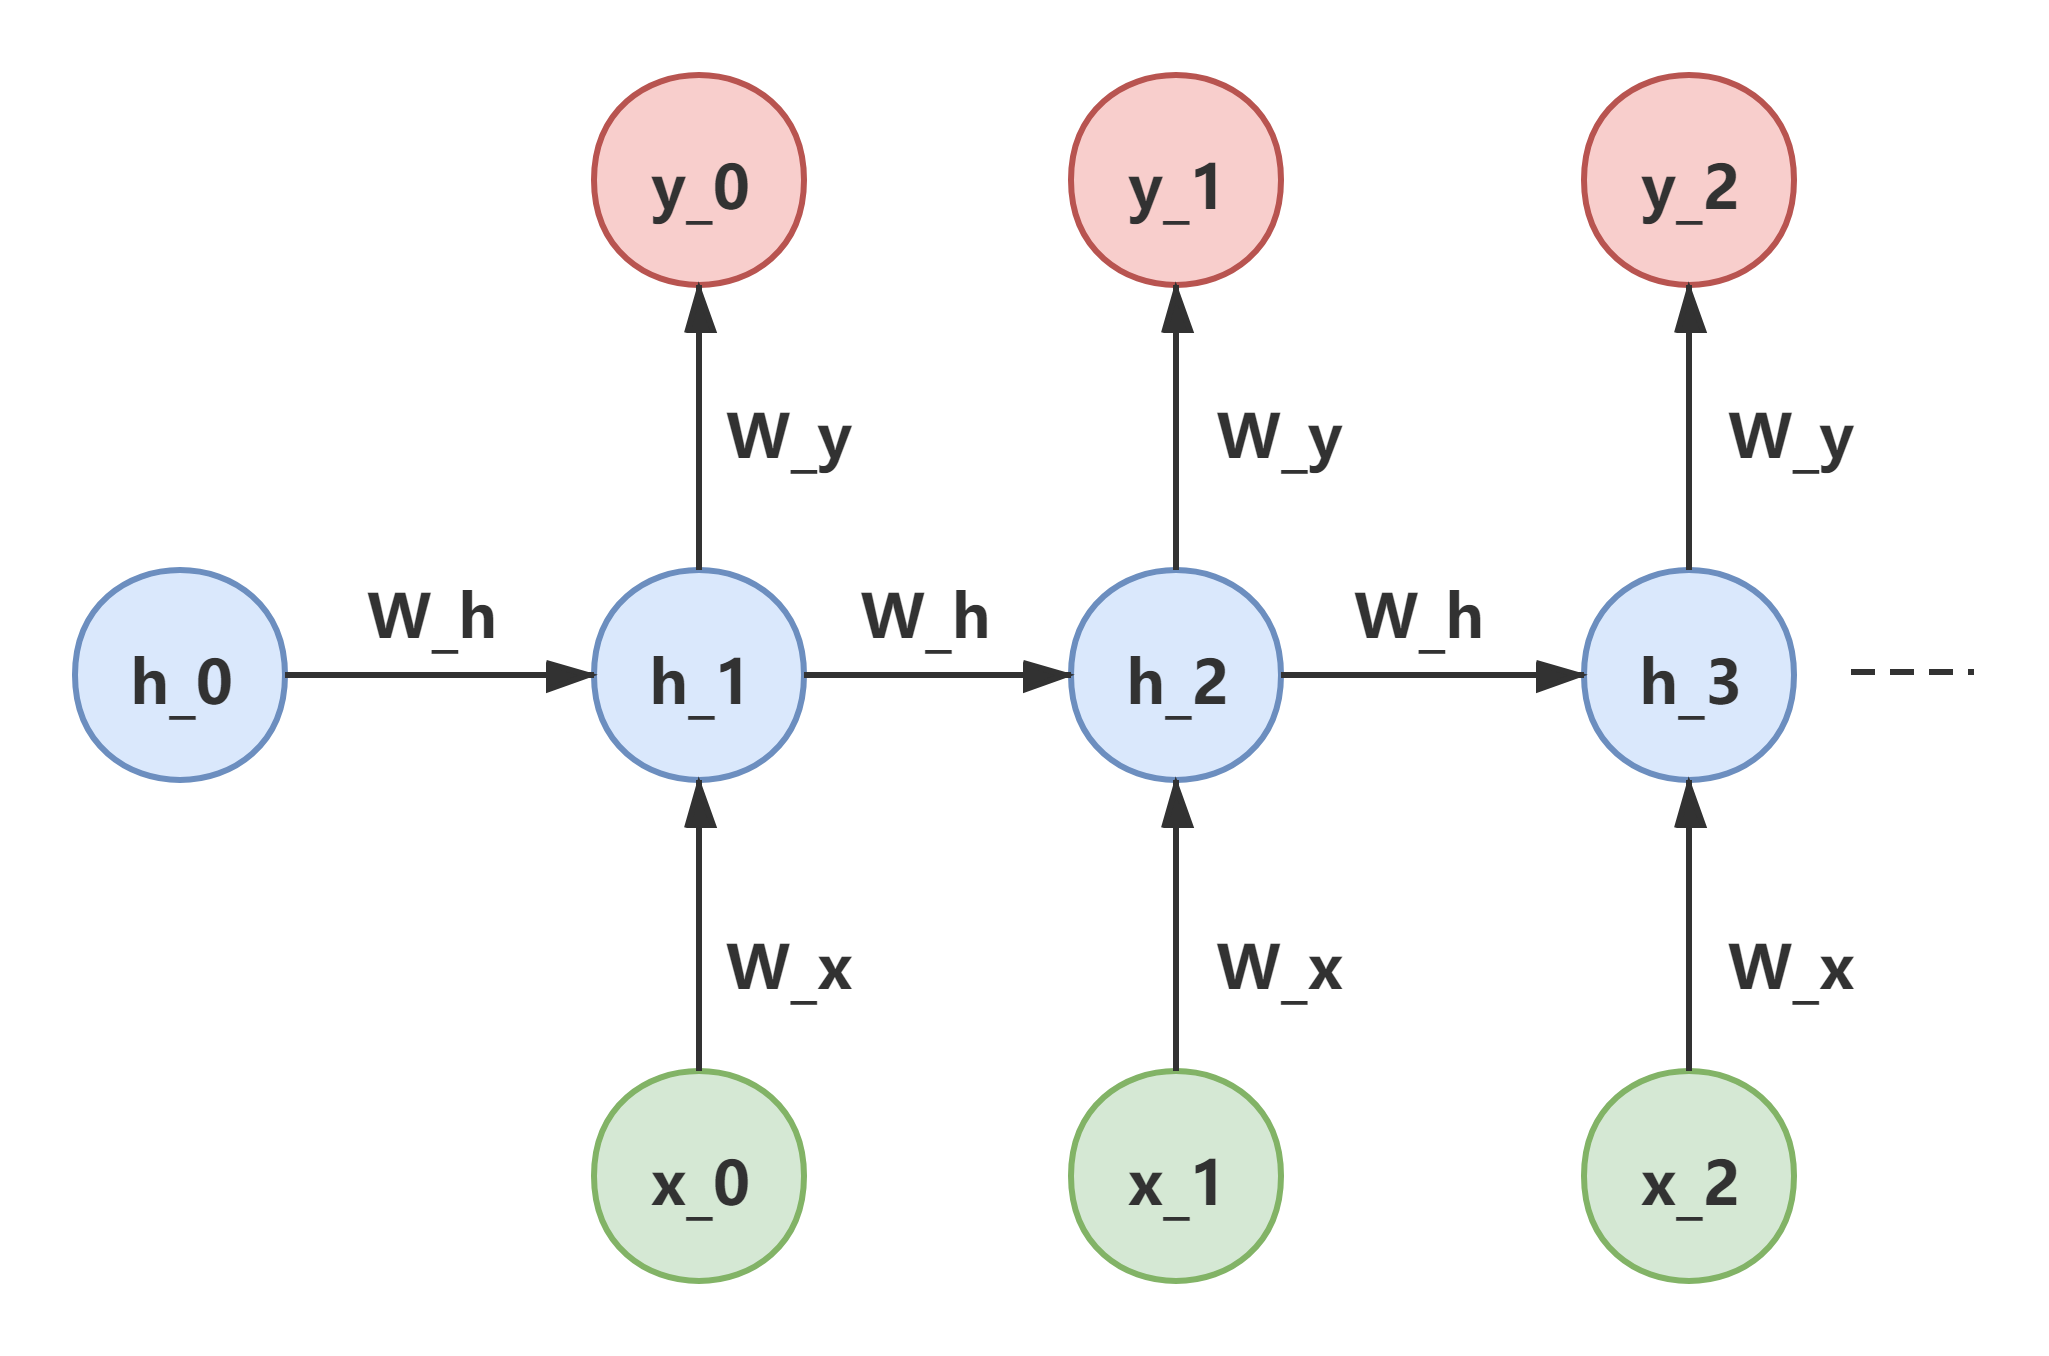
\includegraphics[width=0.9\textwidth]{./images/recurrent-layer-ann.png}
\caption{Recurrent Neural Network}
\label{fig:recurrent-layer-ann}
\end{figure}

\subsection{Backpropagation}

\section{Reinforcement Learning}
\subsection{The Agent–Environment Interface}
The reinforcement learning problem is meant to be a straightforward framing
of the problem of learning from interaction to achieve a goal. The learner and
decision-maker is called the agent. The thing it interacts with, comprising
everything outside the agent, is called the environment. These interact continually, the agent selecting actions and the environment responding to those
actions and presenting new situations to the agent \parencite{Sutton2018}. 
Figure \ref{fig:agent-environment-interaction} diagrams the agent–environment interaction.

\begin{figure}[htbp]
\centering
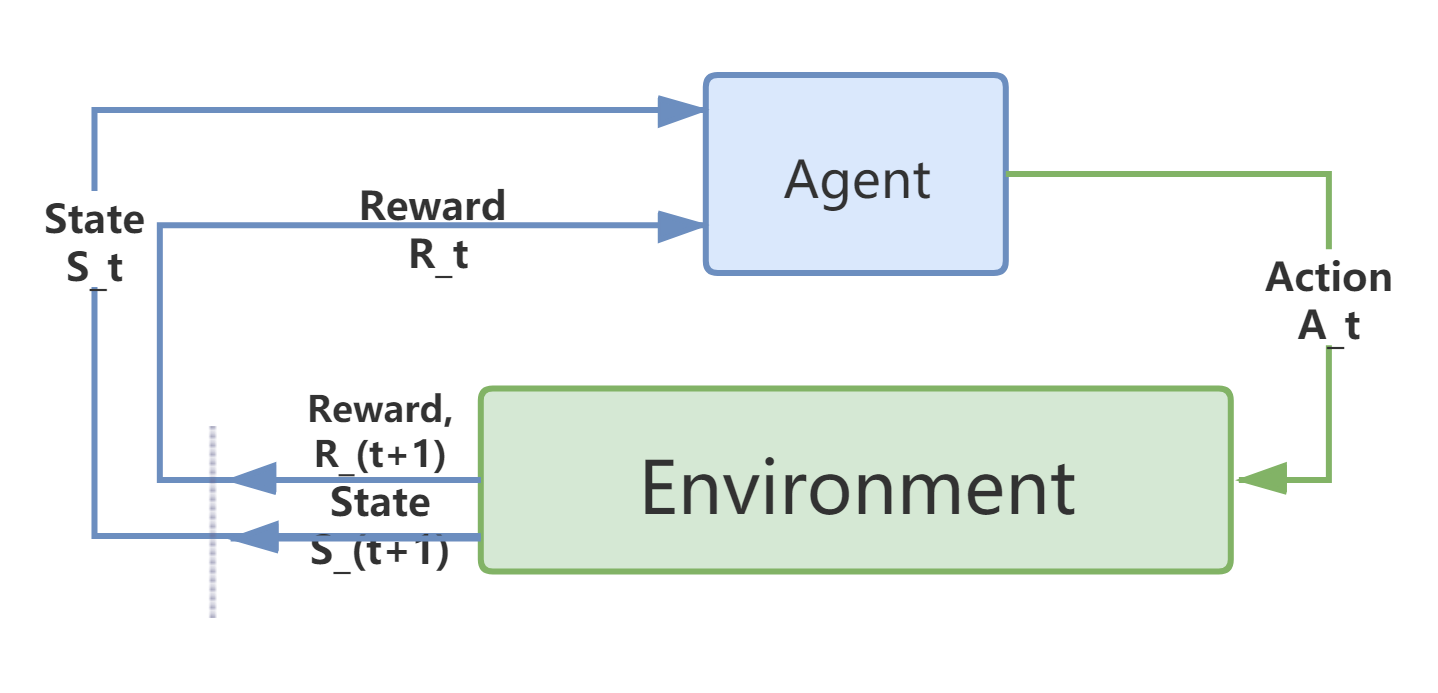
\includegraphics[width=0.5\textwidth]{./images/agent-environment-interaction.png}
\caption{The agent–environment interaction in reinforcement learning, Source: Own illustration based
on\parencite{Sutton2018}.}
\label{fig:agent-environment-interaction}
\end{figure}

Above process is a typical single-agent interaction process. Single agent reinforcement learning algorithms are based on this process. By extending this interactive process, multi-agent interactive process can be intuitively diagrammed In \ref{fig:multi-agent-environment-interaction}. These learning cases are called Multi-Agent-Reinforcement Learning \gls{marl}. In the figure \ref{fig:multi-agent-environment-interaction} agent is splited as two parts perceptor and learner. Perceptors observe the environment and send the state to learners. Learners learn strategies based on the states, rewards and actions. There are many methods, which proposed in these years. Some \gls{madrl} methods will be discussed in following sections. According to the design requirements of the training environment, the structure of the interaction process is flexible.

\begin{figure}[htbp]
\centering
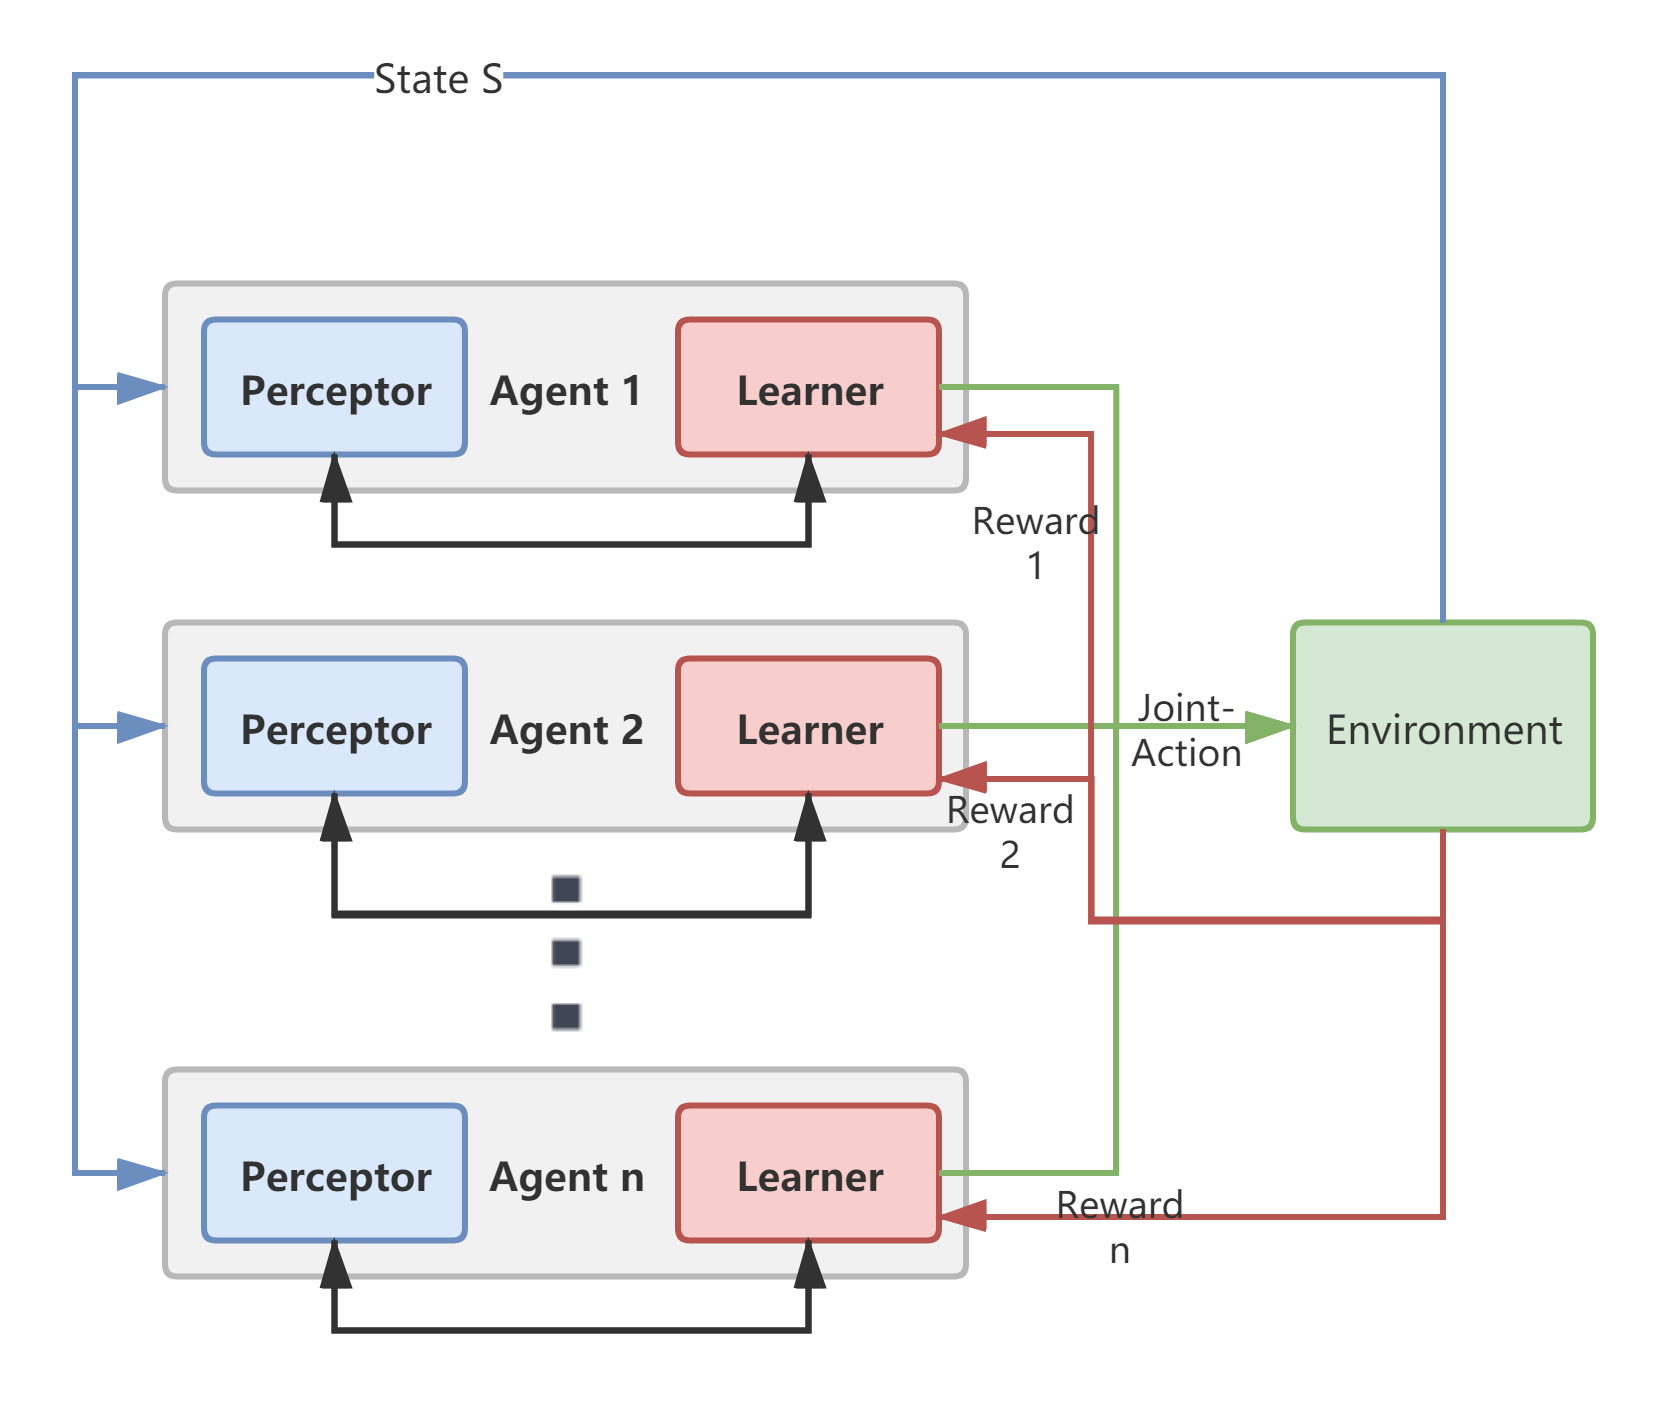
\includegraphics[width=0.6\textwidth]{./images/multi-agent-environment-interaction.png}
\caption{The multi-agent–environment interaction in reinforcement learning, diagrammed In \parencite{en13010123}.}
\label{fig:multi-agent-environment-interaction}
\end{figure}

\subsection{Value Function}
Value Function can be referred as the state-value function and state-action-value-function which consists fixed state or both state and action, respectively.

\textbf{State-Value-Function} measures the goodness of each state. It is based on the return Reward G following a policy Pi. In a formal way, the value of $V_\pi(s)$ is:

\begin{equation} 
V_{\pi}(s)=\mathbb{E}_{\pi}\left[G_{t} \mid s=s_{t}\right]=\mathbb{E}_{\pi}\left[\sum_{j=0}^{T} \gamma^{j} r_{t+j+1} \mid s=s_{t}\right]
\end{equation}

\textbf{Action-Value Function} which measures the goodness of each pair of state, action. Compared with state-value function action is determined.

\begin{equation}
Q_{\pi}(s, a)=\mathbb{E}_{\pi}\left[G_{t} \mid S_{t}=s, A_{t}=a\right]=\mathbb{E}_{\pi}\left[\sum_{j=0}^{T} \gamma^{j} r_{t+j+1} \mid S_{t}=s, A_{t}=a\right]
\end{equation}

\subsection{Bellman Functions}
In summary, Bellman Functions decomposes the value function into two parts, the immediate reward plus the discounted future values. Equation \ref{equation:bellman-state-value-function} show how to recursively the Bellman equation is defined for the state-value function:

\begin{equation} \label{equation:bellman-state-value-function}
V_{\pi}(s)=\sum_{a} \pi(a \mid s) \cdot \sum_{s \prime} P_{s s^{\prime}}^{a}\left(r(s, a)+\gamma V_{\pi}\left(s^{\prime}\right)\right)
\end{equation}

As same as Bellman equation for the state-value function, equation \ref{equation:bellman-action-value-function} tells us how to find recursively the value of a state-action pair following a policy $\pi$.
\begin{equation} \label{equation:bellman-action-value-function}
Q_{\pi}(s, a)=\sum_{s^{\prime}} P_{S S^{\prime}}^{a}\left(r(s, a)+\gamma V_{\pi}\left(s^{\prime}\right)\right)
\end{equation}

\subsection{Q-Learning}
To maximize the total cumulative reward in the long sequence is the goal of Agent. The policy, which maximize the total cumulative reward is called optimal policy formed as $\pi`*$. Optimal State-Action-Value-Function and optimal State-Value-Function are formed as $Q_\pi`*(s, a)$ and $V_\pi`*(s)$, respectively.

\begin{equation}
\mathcal{L}(\theta)=\sum_{i=1}^{b}\left[\left(y_{i}-Q(s, a \mid \theta)\right)^{2}\right]
\end{equation}
\subsection{Policy Gradient \gls{pg}}
\begin{equation}
\nabla_{\theta} J(\theta)=\mathbb{E}_{s \sim p^{\pi}, a \sim \pi_{\theta}}\left[\nabla_{\theta} \log \boldsymbol{\pi}_{\theta}(a \mid s) Q^{\boldsymbol{\pi}}(s, a)\right]
\end{equation}

\subsection{Deep Reinforcement Learning (\gls{drl})}
\subsubsection{Deep Q-Networks}

\subsubsection{Proximal Policy Optimization (\gls{ppo})}
Disadvantage: the distrubition of action changed too quickly, when the reward is always positiv or negative, some possible action will be disapper.
PPO use some contraint tricks to avoid it. such as clip of policy. The loss function based on PPO-clip is as follow.
\begin{equation}
L\left(s, a, \theta_{k}, \theta\right)=\min \left(\frac{\pi_{\theta}(a \mid s)}{\pi_{\theta_{k}}(a \mid s)} A^{\pi_{\theta_{k}}}(s, a), \quad \operatorname{clip}\left(\frac{\pi_{\theta}(a \mid s)}{\pi_{\theta_{k}}(a \mid s)}, 1-\epsilon, 1+\epsilon\right) A^{\pi_{\theta_{k}}}(s, a)\right)
\end{equation} 

\subsubsection{DPG, DDPG, \gls{maddpg}} \label{background:maddpg}

DPG: create a $\mu$ function to determine the action instead the sample in PG.

DDPG: use Actor-Critic model to create target and execute network. a variant of DPG. policy $\mu$ and critic $Q_\mu$ are approximated with deep neural networks.

MADDPG: DDPG used in multi-agents environments.

MADPG
\begin{equation}
\nabla_{\theta_{i}} J\left(\theta_{i}\right)=\mathbb{E}_{s \sim p^{\mu}, a_{i} \sim \pi_{i}}\left[\nabla_{\theta_{i}} \log \pi_{i}\left(a_{i} \mid o_{i}\right) Q_{i}^{\pi}\left(\mathbf{x}, a_{1}, \ldots, a_{N}\right)\right]
\end{equation}

Extension to deterministic policies

\begin{equation}
\nabla_{\theta_{i}} J\left(\boldsymbol{\mu}_{i}\right)=\mathbb{E}_{\mathbf{x}, a \sim \mathcal{D}}\left[\left.\nabla_{\theta_{i}} \boldsymbol{\mu}_{i}\left(a_{i} \mid o_{i}\right) \nabla_{a_{i}} Q_{i}^{\mu}\left(\mathbf{x}, a_{1}, \ldots, a_{N}\right)\right|_{a_{i}=\boldsymbol{\mu}_{i}\left(o_{i}\right)}\right]
\end{equation}

Loss function is 
\begin{equation}
\mathcal{L}\left(\theta_{i}\right)=\mathbb{E}_{\mathbf{x}, a, r, \mathbf{x}^{\prime}}\left[\left(Q_{i}^{\boldsymbol{\mu}}\left(\mathbf{x}, a_{1}, \ldots, a_{N}\right)-y\right)^{2}\right], \quad y=r_{i}+\left.\gamma Q_{i}^{\boldsymbol{\mu}^{\prime}}\left(\mathbf{x}^{\prime}, a_{1}^{\prime}, \ldots, a_{N}^{\prime}\right)\right|_{a_{j}^{\prime}=\boldsymbol{\mu}_{j}^{\prime}\left(o_{j}\right)}
\end{equation}

\subsubsection{Value Decomposition Networks}

\subsubsection{Mixing Network used in \gls{qmix}}

\subsubsection{\gls{qmix}}

\section{Platform and Library}
\subsection{GENIUS}
\textbf{GENIUS:} An integrated environment for supporting the design of generic automated negotiators \parencite{Lin2014}.

\subsection{\gls{negmas}} \label{background:negmas}
\gls{negmas} is an opensource automated negotiation platform, which can model situated simultaneous negotiations such as \gls{scm} which will be discussed separately in detail in the next section \ref{background-scml}. The purpose of this section is to provide an overview of the key components(e.g. Mechanism, World) of the platform

\gls{negmas} is a python library for developing autonomous negotiation agents embedded in simulation environments. The name negmas stands for either NEGotiation MultiAgent System or NEGotiations Managed by Agent Simulations. The main goal of NegMAS is to advance the state of the art in situated simultaneous negotiations. Nevertheless, it can; and is being used; for modeling simpler bilateral and multi-lateral negotiations, preference elicitation , etc \parencite{Mohammad2019}.

\paragraph{\gls{negmas} and Mechanism}
\gls{negmas} has natively implemented five mechanism, Stacked Algernating Offers Mechanism (\gls{saom}), single-text negotiation mechanisms (st) \ref{}, multi-text mechanisms (mt) \ref{}, GA-based negotiation mechanisms\ref{} and chain negotiations mechasnim\ref{}. Among them, \gls{saom} is the negotiation mechanism that is discussed and used in the experiments of this thesis. It has been introduced in detail in section Autonomous Negotiation \ref{background:saom}. At the same time, in the related negotiatioin mechanism packages, some negotiators, such as AspirationNegotiator in negmas.sao, are developed as key part of the packages. These negotiation negotiator will be used as the baseline negotiators in the following experiments.
\paragraph{\gls{negmas} and World}
A simulation is an embedded domain in which agents behave. It is represented in \gls{negmas} by a World. The world in \gls{negmas} was designed to simply the common tasks involved in constructing negotiation driven simulations \ref{}. The entire simulation includes multiple simulation steps which is different with the negotiation rounds. A simulation step can have multiple negotiation rounds. In each step, agents can be allowed to take proactive actions by performing operations worldwide, reading their status from the world, or requesting/operating negotiations with other agents.

The overview of the main components of a simulation in a \gls{negmas} world is shown in Figure \ref{fig:overview-negmas}.

\begin{figure}[htbp]
\centering
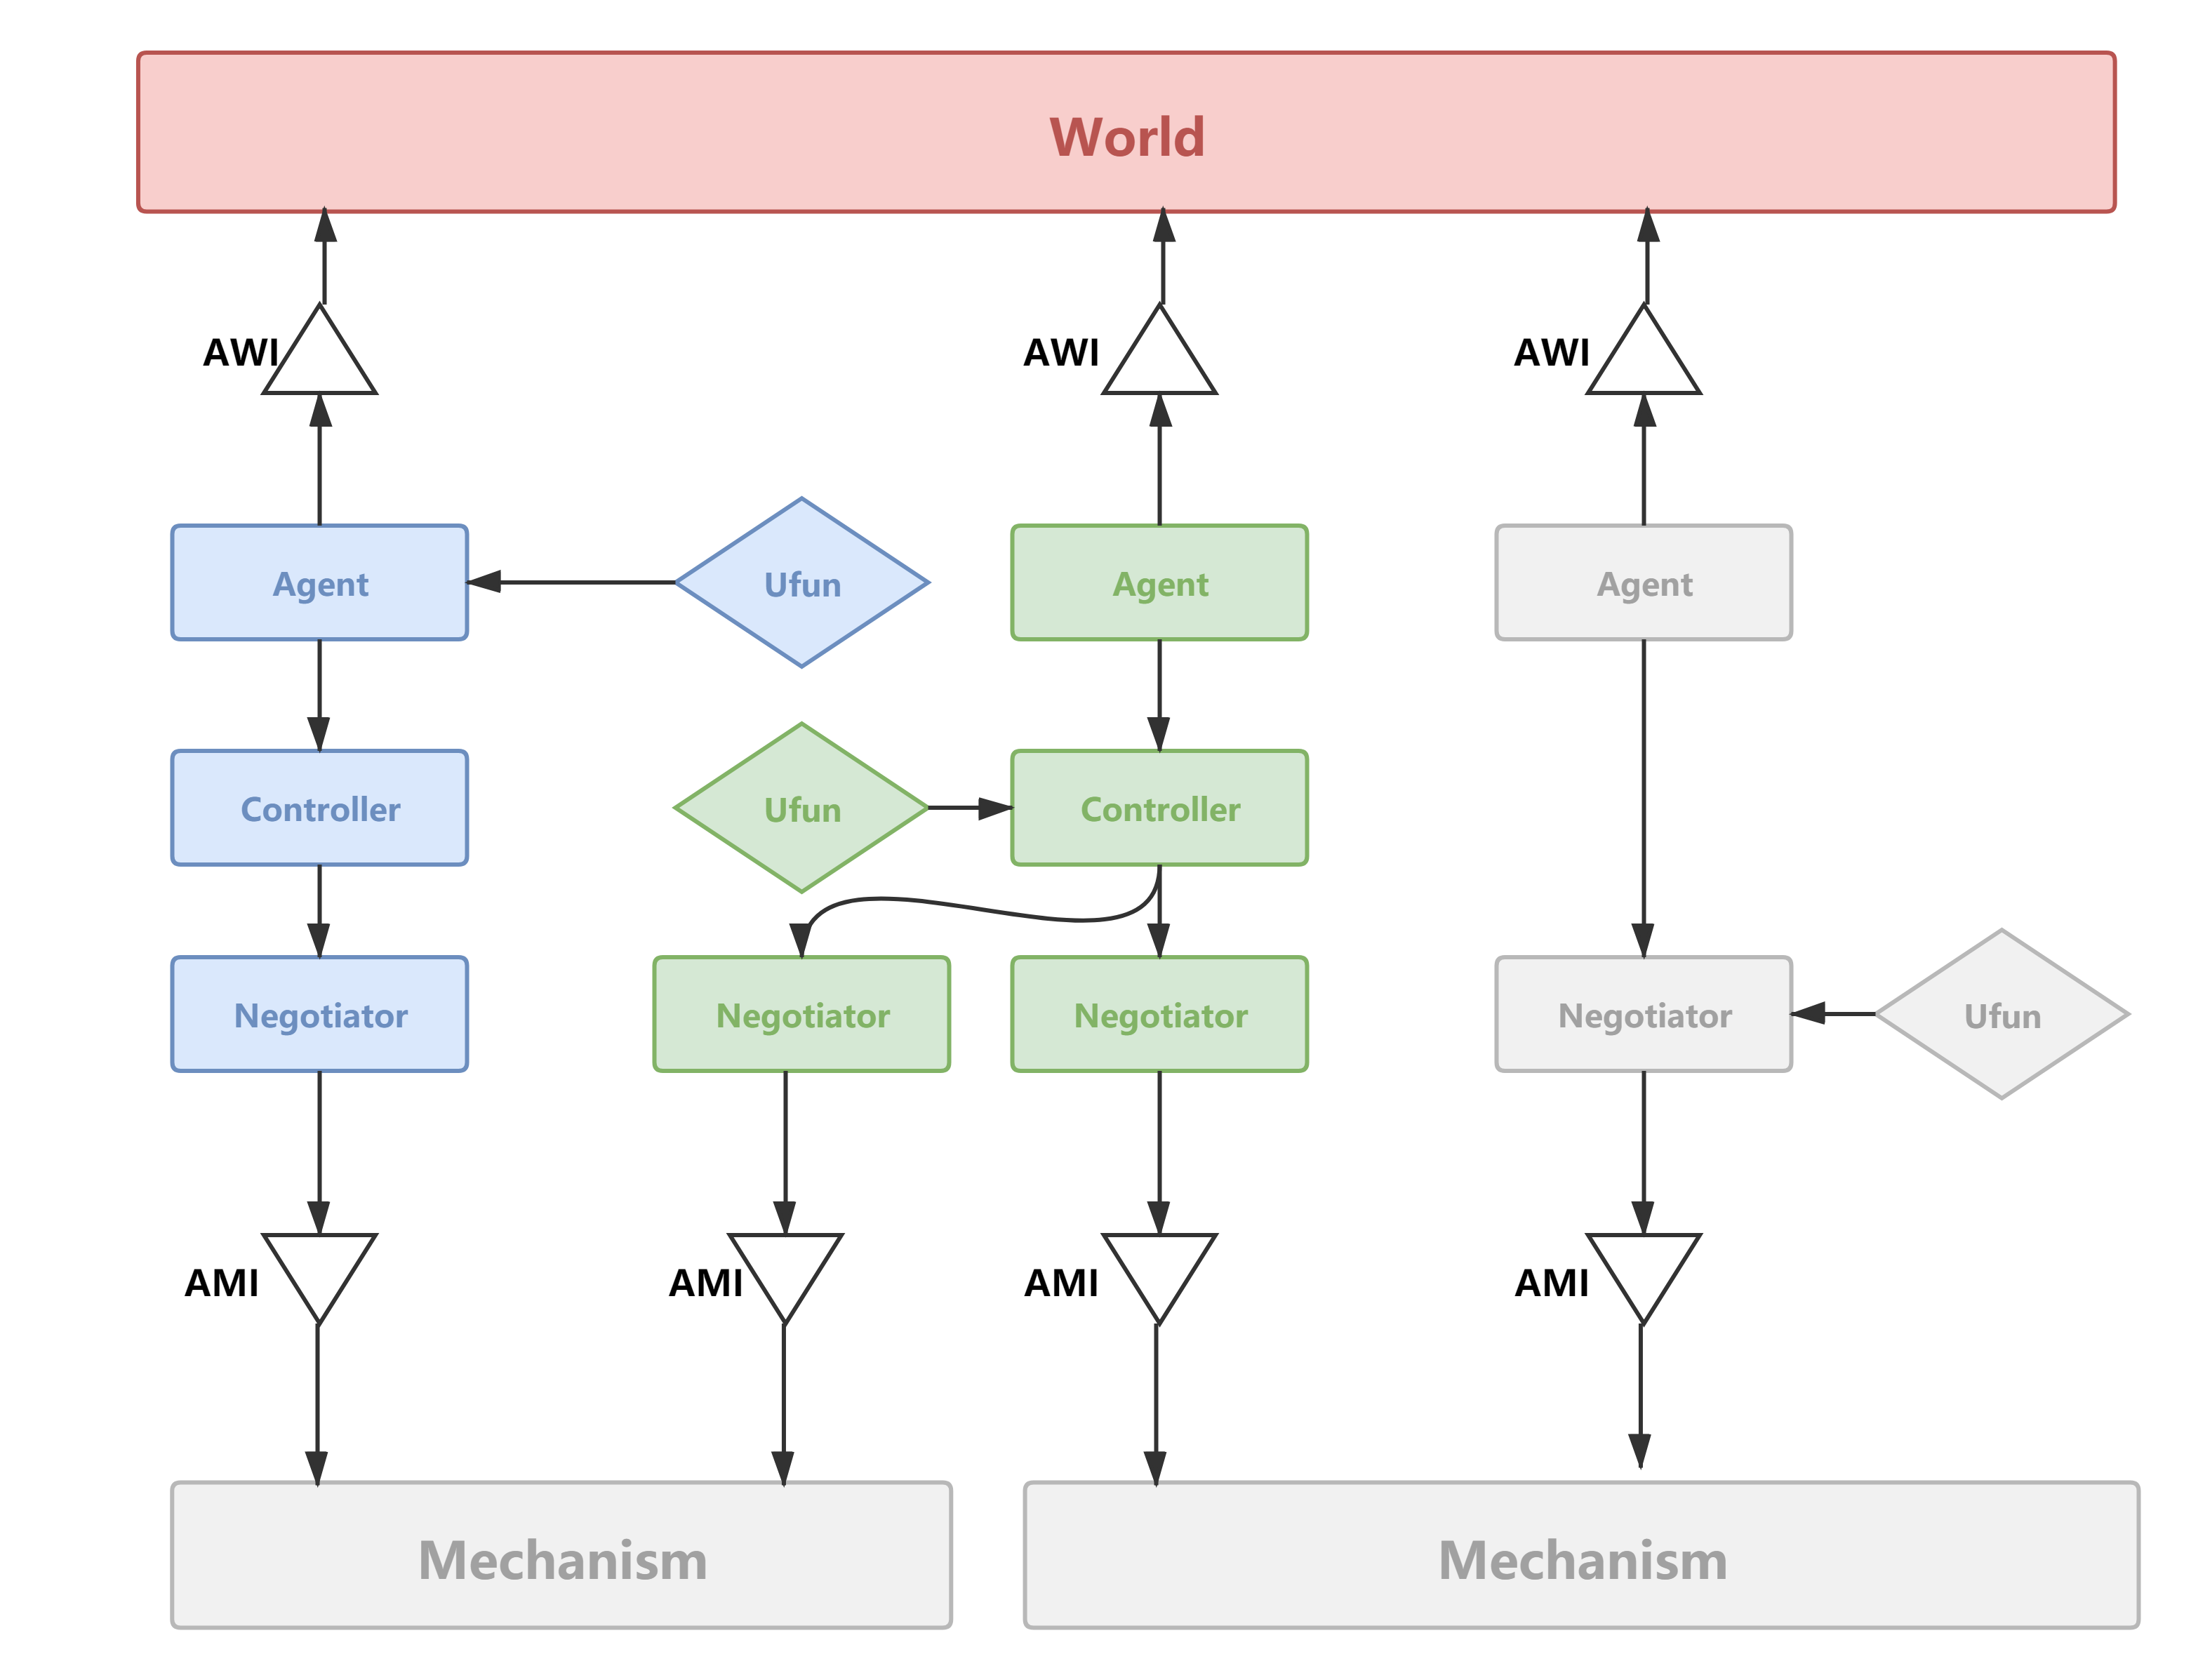
\includegraphics[width=0.8\textwidth]{./images/overview-negmas.png}
\caption{Main components and interactive logic of a simulation in a \gls{negmas} world, Source: Own illustration based on\parencite{Mohammad2019}}
\label{fig:overview-negmas}
\end{figure}

\subsection{\gls{scml}} \label{background-scml}
A supply chain is a sequence of processes by which raw materials are converted into finished goods. A supply chain is usually managed by multiple independent entities, whose coordination is called \textbf{supply chain management(\gls{scm})}. SCM exemplifies situated negotiation. The SCM world was built on top of  \gls{negmas} to serve as a common benchmark environment for the study of situated negotiation \parencite{Mohammad2019}. This repository is the official platform for running \gls{anac} Supply Chain Management Leagues. It will contain a package called scmlXXXX for the competition run in year XXXX. For example scml2019 will contain all files related to the 2019’s version of the competition \ref{}.
There are three main different versions of \gls{scml}, which have different designs. In the following sections, the similarities and differences will be introduced. 

\begin{itemize}
	\item SCML2020-OneShot: Agent Competition (\gls{anac}) Supply Chain Management League OneShot trace (\gls{scml-oneshot}).
	\item SCML2020/2021: Standard Automated Negotiation Agent Competition (ANAC) Supply Chain Management League (\gls{scml}) 2020/2021.
	\item SCML2019: Standard Automated Negotiation Agent Competition (ANAC) Supply Chain Management League (\gls{scml}) 2019
\end{itemize}

\subsubsection{SCML2019}

\subsubsection{\gls{scml}2020/2021}
\gls{scml} was originally developed as a part of \gls{negmas}, from the version ? it was splited as an independent project to research \gls{scm}. \gls{scml} realized a \gls{scm} World to simulate the \gls{scm} process.  

\subsubsection{SCML2020-OneShot} 
In \gls{scml-oneshot} World, the simulation steps can be referred as days. There are multiple concurrent negotiations going on every day. Difference with the SCML2019 and SCML2020/2021, \gls{scml-oneshot} emphasizes negotiation and de-emphasizes operations (e.g. scheduling) which are also important in standard scml. The simulation in oneshot focuses on the the research of concurrent negotiation. The design of \gls{scml-oneshot} ensures the following points \parencite{Mohammad2021}:

\begin{itemize}
	\item Agents (factory managers) consider only the negotiations in the current simulation step. Only the current concurrent negotiations can affect the agent's score. It means, regardless of the result of the negotiations, the concurrent negotiations will be ended at the end of the simulation step. 
	\item Agents can learn over time about their negotiation partners (i.e. suppliers or consumers).
\end{itemize} 

Figure \ref{fig:overview-scml-oneshot} diagrams a World in \gls{scml-oneshot}

\begin{figure}[htbp]
\centering
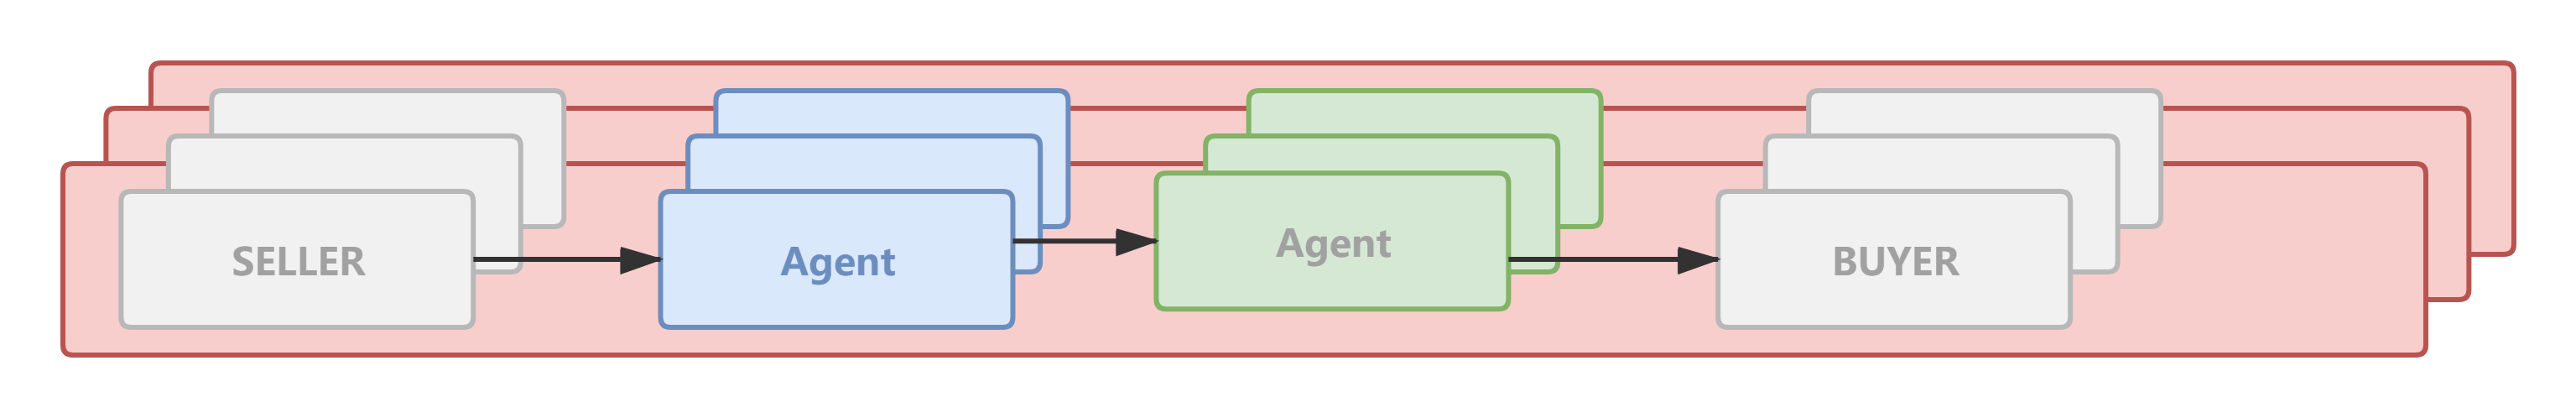
\includegraphics[width=0.8\textwidth]{./images/overview-scml-oneshot.png}
\caption{Main running logic of a simulation in a \gls{scml-oneshot} world, Each red box represents a day. Broken lines represent exogenous contracts while connected lines are negotiations (about the intermediate product). All negotiations conducted in a given day are about deliveries on the same day. Source: Own illustration based on\parencite{Mohammad2021}}
\label{fig:overview-scml-oneshot}
\end{figure}

There are many agents which has same type in the \gls{scm} World. 

Researchers have also developed many negotiation agents such as Agent1[], Agent2[], Agent3[] in GENIUS, Agent4[], Agent5[], Agent6[] in \gls{negmas}.

\subsection{\gls{pytorch}} PyTorch is an open source machine learning library and framework which performs immediate execution of dynamic tensor computations with automatic differentiation and GPU acceleration, and does so while maintaining performance comparable to the fastest current libraries for deep learning. \parencite{NEURIPS2019_bdbca288}. While considering performance, it is also easier to apply and debug.

\subsection{\gls{openai gym}}
\gls{openai gym} is a toolkit for developing and comparing reinforcement learning algorithms \parencite{brockman2016openai}.
\subsubsection{Environment}
The core gym interface is \texttt{Env}, which is the unified environment interface. The following are the Env methods that developers should implement \parencite{brockman2016openai}.

\paragraph{STEP} Run one timestep of the environment's dynamics. When end of episode is reached, \texttt{reset()} is calld to reset this environment's state. Accepts an action and returns a tuple (observation, reward, done, info).
\begin{itemize}
\item observation (object): agent's observation of the current environment, such as frame of the game.
\item reward (float): amount of reward returned after previous action, such as 1 when action is go to left.
\item done (bool): whether the episode has ended, in which case further step() calls will return undefined results, such as agent is dead in game, as True.
\item info (dict): contains auxiliary diagnostic information (helpful for debugging, and sometimes learning), such as goal of agent.
\end{itemize}

\paragraph{RESET} Resets the environment to an initial state and returns an initial observation. This function should not reset the environment's random number generator(s). Random variables in the environment's state should be sampled independently between multiple calls to \texttt{reset()}. Each call of \texttt{reset()} should yield an environment suitable for a new episode, independent of previous episodes.
\paragraph{RENDER} Define how to display the output of the environment. Multiple modes can be used: 
\begin{itemize}
	\item human: Render to the current display or terminal and return nothing. Usually for human consumption
	\item rgb\_array: Return an numpy.ndarray with shape (x, y, 3), representing RGB values for an x-by-y pixel image, suitable for turning into a video.
	\item ansi: Return a string (str) or StringIO.StringIO containing a terminal-style text representation. The text can include newlines and ANSI escape sequences (e.g. for colors).
\end{itemize}

\paragraph{CLOSE} Override close in the subclass to perform any necessary cleanup. Environments will automatically \texttt{close()} themselves when garbage collected or when the program exits. Save datas at the end of the program.
\paragraph{SEED} Sets the seed for this env's random number generator(s). It is useful for reproducing the results.
\begin{lstlisting}[caption={Logic of \gls{openai gym} Interaction},label={lst:openaigym},language=python]
ob0=env.reset() #sample environment state, return first observation
a0=agent.act(ob0) #agent chooses first action
ob1,rew0,done0,info0=env.step(a0) #environment returns observation,
#reward, and boolean flag indicating if the episode is complete.
a1=agent.act(ob1)
ob2,rew1,done1,info1=env.step(a1)
...
a99=agent.act(o99)
ob100,rew99,done99,info2=env.step(a99)
# done99 == True => terminal
\end{lstlisting}

From Listing \ref{lst:openaigym}, user can get the logic of interaction in \gls{openai gym}.

\subsubsection{Stable Baselines}
The stable baselines developed in the project stable-baselines \parencite{stable-baselines}. All implemented algorithms with characteristic discrete/continuous actions are shown in \ref{tab:stable-baselines}.

\begin{table}[htbp]
\centering
\begin{tabular}{l l l} \toprule
\bfseries Name       & \bfseries Box  & \bfseries Discrete \\ \midrule
\verb#A2C#                         & Yes  &  Yes \\
\verb#ACER#                  			 & No   &  Yes \\
\verb#ACKTR#                       & Yes  &  Yes \\
\verb#DDPG#                        & Yes  &  No  \\
\verb#DQN#                         & No   &  Yes \\
\verb#HER#                         & Yes  &  Yes \\
\verb#GAIL#                        & Yes  &  Yes \\
\verb#PPO1#                        & Yes  &  Yes \\
\verb#PPO2#                        & Yes  &  Yes \\
\verb#SAC#                         & Yes  &  No  \\
\verb#TD3#                         & Yes  &  No  \\
\verb#TRPO#                        & Yes  &  Yes \\
\bottomrule
\end{tabular}
\caption{stable baselines algorithms}
\label{tab:stable-baselines}
\end{table}

\subsection{\gls{ray}}
Ray is packaged with the following libraries for accelerating machine learning workloads.
\begin{itemize}
	\item Tune: Scalable Hyperparameter Tuning
	\item RLlib: Scalable Reinforcement Learning
	\item RaySGD: Distributed Training Wrappers
	\item Ray Serve: Scalable and Programmable Serving
\end{itemize}



